\documentclass[12pt]{report}

\usepackage{amsmath}
\usepackage[utf8]{inputenc}
\usepackage[norsk]{babel}
\usepackage{listings}
\usepackage{graphicx}
\usepackage{caption}
\usepackage{verbatim}
\usepackage{float}
\usepackage{pgfplots}
\restylefloat{table}

\title{TMM4850: Prosjektrapport}
\author{Eirik Jakobsen\\ Christopher Tannum}
\date{February 2015}



\begin{document}

\begin{titlepage}
    \begin{center}
        \vspace*{2.5cm}
        
        \Huge
        \textbf{TMM4850: Prosjektrapport}
        
        \vspace{0.5 cm}
        
        \large
        Gruppe E
        
        \vspace{2cm}
        
        
        \Large
        \textit{Christopher Tannum \\ Sindre Raknes \\ Audun 							Stensgaard \\ Tom Meland Pedersen \\ Tor-Håkon 							Bonsaksen}
        
    
    \end{center}
\end{titlepage}


\chapter*{
    \begin{center}
        Abstract
    \end{center}
}

Parallel programming is without a doubt something that any modern programmer needs in his/her toolbox. 
As the physical limits of a single processing unit is reached, parallel computers, both local and distributed are needed to continue to increase processing power. 
OpenMP and MPI are libraries that can be used to develop parallel programs with shared memory(OpenMP and MPI) and distributed systems(MPI).
Even though many serial algorithms can be made fully/partly parallel, the implementation can vary its efficiency.
It is therefor necessary for the programmer to take great care in choosing parallelization techniques for the problem.


\tableofcontents


\chapter{Introduksjon}
Denne rapporten vil gå i dybden og forklare i detalj de ulike aspektene av oppgaven.
Først forklares oppgaven og de forskjellige elementene oppgaven består av. Deretter vil den overordnede arkitekturen bli forklart før alle tre elementene, klient, server og enhet, som prosjektet består av, gås gjennom i detalj. 
Eksempler på hva andre kan lage ved hjelp av APIet vil vises frem og til slutt vil det bli listet opp ting som kan jobbes videre med i fremtiden.


\section{Prosjektbeskrivelse}
Oppgaven gruppen kom frem til var å produsere et bibliotek / API som gjør det mulig og styre Dynamixel servoer[referanse] over ett nettverk. Produktet vi har laget vil hovedsaklig være et verktøy for andre utviklere men vi har laget noen demo applikasjoner for å vise frem hva man kan lage med biblioteket. Problemet med det som eksisterer fra før er at det er proprietært og reduserer muligheten utviklere har når de skal lage programvare som benytter servoene.

\subsection{Dynamixel AX-12}
Dynamixel AX-12 servoene er servoer med dedikerte mikrokontrollere som produseres av Robotis, et Sør-Koreansk selskap. De brukes av hobbyentusiaster og opplæringsinstitusjoner verden rundt til å modellere og simulere roboter, kjøretøyer og andre konfigurasjoner. De er ettertraktet fordi de er billige, robuste og svært fleksible. De er også lette å ta i bruk, mye på grunn av de dedikerte mikrokontrollene som styrer hver individuelle servo.

Grovt forklart har servoene tre input pinner, en for strøm, en for jording og den siste er en seriell datalinje. Hvis man skal ha flere servoer kobles de sammen i serie og de individuelle servoene styres ved at hver enkelt servo har sin unike ID. Servoene drives av en spenning på 9-12 volt.

\begin{figure}[h!]
	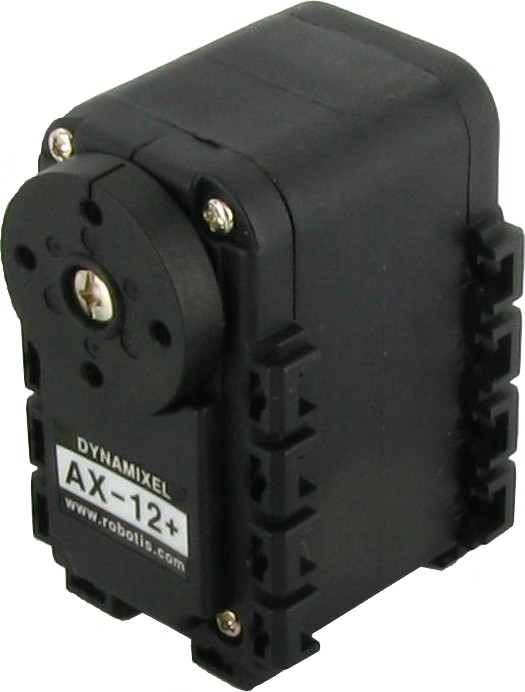
\includegraphics[scale=0.3]{servo_ax12-5}
	\centering
\end{figure}

Dataene som blir sendt gjennom data bussen blir sendt som heksadesimale pakker strukturert som [ref bilde]. På denne måten kan man sette konfigurasjoner som blant annet hastighet og posisjon. Vi kommer ikke til og gå i detalj på hvordan dette fungerer men mer informasjon kan finnes i Dynamixel AX-12 manualen [ref].

\subsection{Bruksområder}
Det som finnes av offisiell støtte for Dynamixel AX-12 servoene fra før er proprietært, og har ikke åpen kildekode. Dette gjør det vanskelig for utviklere og lage egen programvare, spesielt over nettverk. Programvaren vi utvikler vil åpne opp og gjøre det enklere for andre utviklere og lage spennende og sammfunnsnyttige applikasjoner. 

Løsningen åpner for et stort antall videre utviklingsområder. I hovedsak så er det læringsinstitutter som vil kunne ha nytte av det vi lager. Studenter ved neste års Instrumentering og styring over internett, har stor kreativ frihet til å enten bygge videre eller lage noe helt nytt. 

\begin{itemize}
	\item Feste på et kamera og bruke det til å innhente informasjon.
	\item Kan utforske steder som er dårlig egnet for personer.
	\item Kan lage andre ting enn kjøretøy - Sluser, fjernstyrte servoapplikasjoner.
\end{itemize}

\clearpage

\chapter{Arkitektur}
Dette avsnittet beskriver arkitekturen og er ment å gi en overordnet oversikt over de forskjellige delene av prosjektet og hvordan de henger sammen. Mer detaljerte beskrivelser av de forskjellige delene kommer senere i rapporten.

\section{Server-Klient Arkitektur}
Bildet[ref] viser hvordan de forskjellige elementene i prosjektet henger sammen. Punkt 1 er selve enheten som består av en Raspberry pi[ref] som er koblet til servoene. Denne enheten kommuniserer med en ekstern server (2) gjennom sockets[ref]. Serveren (2) håndterer alt av forbindelser mellom brukere og enhetene. Når en enhet kobler seg til vil den registrere seg med et navn, dette navnet kan så benyttes av brukere for og kommunisere med enheten. Del 3 av prosjektet er selve brukeren. Det kan være alt fra en applikasjon på telefon til kontroller styring. Applikasjonen pakker instruksjoner inn i JSON[ref] og sender det til serveren. Serveren sjekker at formatet er riktig strukturert og sender det videre til riktig device.

\section{Andre Mulige Arkitekturer}
Det var flere forskjellige typer arkitekturer som ble vurdert før vi startet utviklingen av prosjektet. Arkitekturene ble sammenlignet med at vi listet positive og negative egenskaper med tanke på oppgaven og hva vi ønsket og oppnå. Til slutt satt vi igjen med en arkitektur som gruppen mente fungerte best til prosjektet.

\subsection{Klient-Enhet}
I denne arkitekturer fungerer enheten som en server og all kommunikasjon går direkte mellom klienten og enheten. Fordelen med en sånn type arkitektur er at den er relativt simpel og utvikle da den fjerner ett ledd. Det vil også bli mindre forsinkelse på kommunikasjonen mellom dem. Den største ulempen med denne typen arkitektur er at enheten ikke nødvendigvis har mulighet til og sette statisk IP (avhenger av nettet man er koblet til) og det kan bli problematisk for brukere og koble seg til den.

\subsection{Klient-Server, Enhet med delt server software}
Denne arkitekturen er ganske lik den vi har valgt men i steden for og ha et dedikert program for serveren og et dedikert program for enheten så er det samme programvare. Det vil si at at programvaren selv detekterer - eller blir konfigurert - for å være server eller enhet og så hånderer den signalene deretter. Fordelen med å gjøre det på denne måten er at det blir mindre å tenke på for folk som skal sette det opp. Ulempen er at det blir mye mer krevende og komplisert å utvikle da det blir vanskeligere å fordele og holde styr på arbeidsoppgaver og ansvarsområder siden man i praksis utvikler to deler i samme programvare.

\section{Arkitekturvalg}
\textbf{Fordelene} med den arkitekturen vi valgte er at det er en ganske standard måte å løse lignende utfordringer på. Det gjør at det er godt dokumentert og enkelt å finne informasjon om det hvis det oppstår problemer. En annen fordel er at man slipper og hente ut IP adressen manuelt fra enheten og man kan forholde seg til ett endepunkt. Enheten vil bare registrere seg på serveren og så kan sluttbrukeren nå enheten gjennom serveren. Denne løsningen er også den beste for å støtte flere brukere og flere enheter, siden man får ett felles kontaktpunkt hvor man kan håndere det. Alle punktene over gjør det mye mer brukervennlig for sluttbrukere å bruke systemet.

\textbf{Ulemper} med denne type arkitektur går mest på utviklingen. Det blir flere deler som skal utvikles og vedlikeholdes og det krever mer kompetanse av utviklerne. Kompleksiteten er også høyere i forhold til og bruke en Klient - Enhet arkitektur men alle de positive sidene på brukeropplevelsen veier opp for de ekstra utfordringene under utviklingen.


\chapter{Enhetslaget}
Enhetslaget består av selve enheten som i vårt tilfelle er et simpelt kjøretøy bygd opp av fire servoer, en raspberry pi med programvaren som styrer servoene, og batteri pakker for både servoene og raspberry pi’en for og få alt trådløst.

\section{Maskinvaren}
Tidlig i prosjektfasen diskuterte gruppen flere muligheter for maskinvare som kunne brukes til å kjøre kontrollprogramvaren. Ønsket var å bruke maskinvare som var lett tilgjengelig, godt dokumentert, brukervennlig og så billig som mulig, men samtidig pålitelig og fleksibel nok til å gi brukere god kontroll over lavnivå funksjonalitet. 

\subsection{Hjernen}
Gruppen vurderte først en Arduino modell da det er en godt kjent og dokumentert platform, de er i tillegg billige og bruker lite strøm noe som gjør dem ideelle til batteridrevne enheter. De krever desverre ekstra maskinvare for å kunne støtte wifi (noe vi så på som essensielt), dette førte til at valget falt på å benytte en Raspberry pi modell. Disse er noe dyrere enn de fleste Arduino produkter, men er mye mer fleksible og brukervennlige, de er godt dokumentert og har et stort brukersamfunn. De bruker generelt mer strøm enn Arduino moduler, men man kan benytte Raspberry pi moduler beregnet for lavt strømforbruk[REFERANSE] dersom dette er ønskelig, ettersom et gruppemedlem allerede hadde en b+ modell tilgjengelig ble det vedtatt å benytte denne til tross for at det gir mindre batterilevetid.

\subsection{Wifi}
For å gi Raspberryen støtte for wifi ble det benyttet en wifi USB-dongle av typen edimax[REFERANSE]. Denne var enkel å installere da Raspbian (det Linuxbaserte operativsystemet til Raspberry pi) allerede støttet den, og dermed krevde den minimalt med konfigurasjon, noe som gjør den svært brukervennlig. Den bruker også svært lite strøm, noe som er ideelt for batteridrevne enheter. I teorien kan man benytte seg av hvilken som helst wifi dongle, så lenge den støttes av det valgte operativsystemet.

\subsection{Servo oppkobling}
Dynamixel bussen kommuniserer med Raspberryen gjennom USB porten via en kommersiell adapter [REFERANSE]. Kontroll-programvaren detekterer selv antall servoer tilkoblet bussen og er designet for å gi “plug and play” funksjonalitet. Som batteripakke til Raspberryen ble en strømbank av typen Ye! Energy Mini [REFERANSE] koblet til mikroUSB inngangen på Raspberryen. Servoene fikk strøm fra den komersielle Dynamixel batteripakken. Merk at disse batteripakkene lett kan byttes ut med andre alternativer så lenge de leverer riktig spenning og har rimelig energikapasitet da batteritilkoblingene er svært generelle og bruker standariserte tilkoblinger. Det er også mulig å koble både Raspberryen og servoene til samme batteripakke, men dette vil kreve ekstra maskinvare i form av strømforsyning og spenningsregulator. Dette vil kunne gjøre systemet mer kompakt, men vil legge til en økt kompleksitet av maskinvare.

\section{Programvaren}
Vi vurderte i begynnelsen å skrive vårt eget lavnivåbibliotek, hovedsakelig for å kunne eliminere bruken av en komersiell adapter mellom Raspberry pi’en og Dynamixel bussen. Det ble raskt oppdaget at dette ikke var praktisk mulig på grunn av strukturen til bussen samt alle de potensielle feilkildene det ga opphav til. Det ville blant annet ha krevd en egen tri-state buffer for å gjøre det mulig å kommunisere med bussen over UART, noe som ville ha økt maskinvare kompleksiteten og satt større krav til maskinvarekonstruksjon for eventuelle fremtidige brukere.

Bruk av den komersielle adapteren førte til at programvaren kun trengte å kommunisere med en standard USB port, noe de aller fleste operativsystemer allerede har driverstøtte for. Dermed kunne programvaren i teorien struktureres slik at den kunne kjøre på en hvilken som helst maskinvare platform med USB porter og støtte for en Linux distribusjon, noe som ble et av hovedmålene med programvaren.

\subsection{Språk}
Tidlig i prosjektperioden satt gruppen krav til programvaren på enheten. Det viktigste var at programvaren skulle være enkel å forstå og være fleksibel på mange områder. I tillegg til dette skulle det være mulig å kjøre programvaren på mange ulike plattformer. Ut i fra kravene kunne gruppen valgt å benytte seg av python eller C. 

Fra tidligere erfaringer ble det naturlig for gruppen å velge å skrive et API i python, som videre kommuniserer med Dynamixel bussen gjennom USB porten. ++++++++
(Prøvde å begynne å skrive om) 
Kravene for programvaren på enheten var at den skulle være enkel og sette seg inn i og fleksibel. I tillegg er det viktig at programvaren kan kjøre på så mange platformer som mulig. De språkene som hadde god støtte for den type funksjonalitet vi var ute etter fra før var python og C, og for enkeltheltskyld valgte vi og bruke python.

Dette gjorde at valget falt naturlig på å skrive et python API som kommuniserte med Dynamixel bussen gjennom en USB port der en kommersiell USB-RSA adapter av typen ………. [REFERANSE] var koblet til bussen. Standardprotokollen for kommunikasjon med Dynamixel aktuatorene ble benyttet, den er godt dokumentert i databladene til servoene [REFERANSE]. 

Python API’et bygger videre på Ian Danforts implementasjon av Dynamixel protokollen i python som igjen er en python versjon av C\# biblioteket skrevet av Patric Goebel.

\subsection{Operativsystem}
Vi benyttet operativsystemet Raspbian som er et Linuxbasert operativsystem tilpasset Raspberry pi. Fordelene ved å benytte et operativsystem er at mye av lavnivå maskinvareaksessering abstraheres bort av eksisterende drivere til både WiFi og USBportene. Ulempene er at det krever mer spesifikk maskinvare, dermed vil systemet bli mer avhengeig av at man benytter seg av den nevnte maskinvaren. Dette kravet blir noe lettet ved at Raspian er basert på Linux kernelen. Dermed vil man i teorien kunne kjøre programvaren på en hvilken som helst Linux distribusjon med en fungerende Python interpreter, f.eks. kan man bruke Embedded Linux dersom man ønsker å konstruerere egen maskinvare.

\subsection{Maskinvare}

\begin{itemize}
	\item Maskinvare detaljer:
	\item Raspberry Pi:
	\item Stømforsyninger:
	\item Adapter:
	\item Programvare detaljer:
	\item Python implementasjon:
	\item Linux konfigurasjon:

\end{itemize}

\clearpage

\chapter{Serverlaget}
For å ha en forbindelse mellom bruker og enhet er det nødvendig med en server. Serveren sin oppgave i dette prosjektet er å mate enheten med kommandoer som brukerapplikasjonen sender. Den har også oppgaven med å håndtere flere enheter som er tilkoblet og all relevant informasjon om enhetene(koblingsobjekt, navn, id). Grunnen til at en server trengs er at enheten kan flyttes over flere nettverk og vil aldri ha en statisk ip adresse. Enheten kan da koble seg opp til en server som håndtere all kontakt mot brukerapplikasjoner. I prinsipp kunne en enhet ha koblet seg direkte opp mot brukerapplikasjonen, men dette vil komplisere bruken av flere enheter betraktelig. Serveren vil også kunne brukes mer aktivt i fremtidige utvidelser, ved for eksempel lagring av statistikk om enheten, samt håndtere feilmeldinger og skape et mye enkelere sett av kommandoer som brukeren må forholde seg til.

\section{Teknologi}
Teknologien som blir brukt som utforming av serveren er Node.js[REF]. Node.js er en platform som er bygd på Chrome sin javascript runtime for å lett bygge raske, skalerbare nettverksapplikasjoner. Grunnen til at denne teknologien ble valgt et først og fremst at det er svært enkelt sette opp en enkel server, samt at Node.js tilbyr enkel interaksjon mot brukerapplikasjoner. 

[WEBSERVER KODEEKSEMPELBILDE]

\section{Serveroppbygning}
Serveren er bygd opp av tre moduler. En mastermodul som håndterer instansiering av serveren, en modul for koble opp mot enheten, og til slutt en modul for å koble opp mot brukerapplikasjoner. 

[RELEVANT SKILDRING AV MODULENE]

\subsection{Mastermodul}
Mastermodulen importerer alle aktuelle bibliotek som brukes (se tabell [ref]). I tillegg lager den en HTTP server som brukerapplikasjoner tar i bruk, samt setter opp en socket som kobles opp mot enheten(e).

\subsection{Socketmodul}
Modulen for å koble opp mot enheten er en socketserver. Socketserveren består av funksjoner som håndterer events fra enheten samt et sett av hjelpefunksjoner. Events som socketserveren håndterer er: når en enhet kobler seg til serveren, når data blir sendt fra enheten og når enheten kobler seg fra serveren. Når en enhet kobler seg til serveren skjer det i praksis ingenting, det er først når enheten sender nødvendig informasjon om seg selv at koblingen kan bli tatt i bruk. Grunnen til at det blir gjort på denne måten er at brukeren senere skal kunne bruke f.eks. navnet til enheten han/hun skal styre. Når enheten har sendt sin informasjon til serveren gjennom en socket, lages et koblingobjekt som blir lagret sammen med dens navn samt en unik id som serveren genererer. På denne måten kan flere enheter koble seg til serveren, der hver enhet får et unikt koblingsobjekt. Når en enhet kobler seg fra serveren så vil all aktuell informasjon om enheten fjernes fra serveren. Hjelpefunksjonene ble konstruert for å enkelt hente ut id, koblingsobjekt og navn til en aktuell enhet. Det eksisterer også en hjelpefunksjon for å generere id til nye enheter som kobler seg på. 

\subsection{Restmodul}
Modulen for å koble opp mot brukeren er en http-server. Http-serveren genererer et REST-API mot brukeren. Serveren sitter og lytter på brukerforespørsler basert på HTTP URL-en. Avhengig av hvilken forespørsel brukeren sender, så sendes enten informasjon direkte til enheten basert på koblingsobjektet og id, eller så returneres aktuell informasjon direkte til brukeren uten å gå innom enheten. For eksempel en brukerforespørsel om en gitt enhets id, vil bli sendt direkte fra server til brukerapplikasjonen uten å gå innom enheten. HTTP-serveren er koblet opp mot socket-serveren ved at	den importerer socket-servermodulen og behandler det aktuelle koblingsobjektet til enheten.


\begin{table}[H]
	\begin{tabular}{|c|c|}
		\hline 
		\textbf{Bibliotek }& \textbf{Informasjon} \\ 
		\hline 
		Express.js &   \\ 
		\hline 
		Net &  \\ 
		\hline 
		JSON &  	\\ 
		\hline 
		BodyParser &  	\\  
		\hline 
	\end{tabular} 
	\centering
	\caption{Bibliotek brukt på server}
	\label{timing_4096}
\end{table}

\chapter{Endepunkter}
For å demonstrere og teste APIet har vi laget to applikasjoner med forskjellig teknologi.
Den første er en enkel nettside som lar brukeren styre et kjøretøy og som viser en del sanntidsinformasjon om enheten, som f.eks fart, temperatur og annen status informasjon. Den andre demo applikasjonen er en java applikasjon som lar brukeren styre enheten med en Playstation eller Xbox kontroller.

\section{Kontrollpanel}
For å demonstrere hvordan og hva man kan bruke APIet til har gruppen laget en enkel web applikasjon som lar brukeren styre et kjøretøy gjennom nettleseren sin. Dette fungere som et enkelt kontrollpanel og kan brukes på både mobiltelefon og desktop. Siden består i hovedsak av to slidere, en som styrer hastighet og en som styrer retning/svinging. I tillegg til enkle brytere for og styring er det en tabell som viser live informasjon fra en servo. Dette er for å demonstrere hva slags informasjon som er tilgjengelig for sluttbruker.

[BILDE]

\subsection{Utvikling}
Nettsiden er utviklet i standard HTML5, javascript og CSS [Ref?]. Foundation [Ref] blir brukt for å gjøre siden responsiv, det vil si at samme siden kan kjøre og se bra ut på forskjellige skjermstørrelser, noe som gjør at man ikke trenger å kode en egen versjon for telefoner og nettbrett. jQuery[ref] og jQuery Speedometer[ref] brukes for å lage et speedometer som viser farten til kjøretøyet.

\section{Kontroller applikasjon}
Dette er den andre av to applikasjoner som gruppen har utviklet. Denne tar input fra en Playstation eller Xbox kontroller, pakker det inn i JSON og sender det til serveren. For og demonstrere bil-abstraksjonslaget styrer kontrolleren kjøretøyet ved og akslerer og styre svinging med joystickene, på samme måte som de fleste videospill gjør. Dette gjør at det føles ganske naturlig og styre kjøretøyet for de som har spilt videospill før.

\subsection{Utvikling}
Dette programmet er utviklet i Java 1.8[ref]. For å håndtere kontroller input brukes biblioteket jGamepad[ref]. Det siste biblioteket som brukes er GSON[ref] som konverterer objekter til JSON som kan sendes og bli håndert av serveren. Komunikasjonen til serveren foregår ved at applikasjonene lager en HTTP pakke, med all relevant informasjon fra kontrolleren, og sender det til serveren.

For å kunne bruke en Playstation 3 kontroller med programmet må man emulere en Xbox kontroller med programvare som for eksempel XInput Wrapper[Ref]. Grunnen til dette er at XBOX kontrollere er offisielt støttet av Windows med egne drivere mens Playstation 3 kontrollere ikke har noen støtte.

\clearpage

\chapter{Videre arbeid}
Det var en del ønsket funksjonalitet gruppen ikke fikk tid til og implementere i dette prosjektet.

\section{Støtte for sensorer}
Vi hadde tilgang til en Dynamixel Sensor Module AX-S1[ref] og med litt mer tid så kunne vi utviklet støtte for de også. De er veldig sentrale i mange konfigurasjoner, spesielt de som er laget for og gjøre ting automatisk uten å styres eksternt (Autonomt).

\section{Eksponere lav-nivå funksjonalitet}
Det var planlagt å gjøre det mulig å sette enkelt verdier på servoene som for eksempel led lys, torque og mange andre. Utfordringen her er at hvis sånne verdier blir satt ufiltrert kan det skade, eller til og med ødelegge servoene. På grunn av disse utfordringene og mangel på tid bestemte vi oss for å bare støtte noen få, som for eksempel hastighet og posisjon.

\section{Abstraksjonslag for robot}
Vi utviklet et abstraksjonslag for å gjøre det enkelt for en sluttbruker å styre et kjøretøy med hjul. Det som kunne vært interessant er å lage ett abstraksjonslag til som gjør det samme for roboter med to bein som skal bevege seg. Det er lagt inn støtte for og gjøre det lett og implementere dette i fremtiden for eventuelt andre som vil bygge videre på prosjektet.

\section{Logging og statistikk}
Loggingen på serveren er litt mangelfull. For å gjøre det enklere å feilsøke for andre utviklere ville det vært en fordel om det var litt mer detaljert. Det hadde også vært interessant å holde oversikt over statistikk.

\section{Bruddhåndtering}
Det er mye som kan gå galt med forbindelsen når man har tre ledd som all informasjon skal igjennom. Det er ingen sikkerhetsmekkansime på enheten som gjør at de stopper hvis forbindelsen blir brutt. Dette vil si at hvis noen kjører enheten og den mister forbindelse vil den bare fortsette med den farten og retningen den hadde.

Et annet problem hvis enheten mister forbindelse er at serveren ikke har støtte for koble seg på samme ID. Det vil si at alle endepunktapplikasjoner selv må håndtere slike brudd og oppdatere sin informasjon for og få enhetens nye ID.

\section{Sikkerhet og autorisasjon}
Det er mange sikkerhetsaspekter som ikke har blitt prioritert under utviklingen. Selv om at det er mulig å være mange brukere og enheter på systemet samtidig er det foreløping ingenting som hindrer en bruker fra å styre en annens persons enhet eller gjøre andre potensielt uheldige ting. Dette kan løses ved å introdusere brukerautorisasjon og knytte enheter til brukere eller en gruppe med brukere. 

\clearpage

\chapter{Konklusjon}
Det fungerer
Noen mangler men det er greit
Klarte mye på lite tid
Resultatet er tilfredstillende



\begin{figure}[H]
	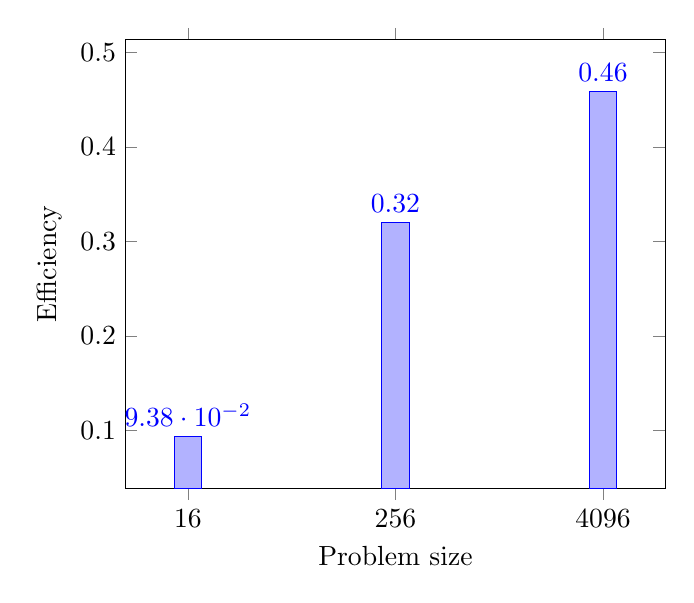
\begin{tikzpicture}
		\begin{axis}[
		  ybar,
    enlargelimits=0.15,
    legend style={at={(0.5,-0.15)},
      anchor=north,legend columns=-1},
    ylabel={Efficiency},
    xlabel={Problem size},
    symbolic x coords={16,256,4096},
    xtick=data,
    nodes near coords,
    nodes near coords align={vertical},
		]
	\addplot 
		coordinates {(16,0.09375) (256,0.32)
			 (4096,0.4588254866) };	
	\end{axis}
	\end{tikzpicture}
	\centering
	\caption{Efficiency as problem size grows.}
	\label{scaling}
\end{figure}



\end{document}